% -*- Mode:TeX -*-
%% Yonsei University Graduate School thesis — root document.
%% Layout follows the official 2026 English doctoral Word sample
%% ("영문 MSword_박사학위논문_양식_2026.docx"). Per-thesis metadata lives
%% in thesis.json (rendered into front/cover.tex, signature.tex and
%% titlekor.tex by scripts/build.sh). On Overleaf edit those three files.
%%
%% Page order (spec "Order of Manuscript"):
%%   Cover / Title / Signature / Acknowledgements / TABLE OF CONTENTS (i)
%%   / List of Figures / List of Tables / Abstract / Text (1, 2, 3 ...)
%%   / Appendices / References / Abstract in Korean

\documentclass[10pt]{mitthesis}   % 10pt (as in the Word sample) or 11pt per spec

%% NOTE: mitthesis.cls already loads amsmath, amsthm, newtxtext/newtxmath
%% (Times), caption, geometry, setspace, CJKutf8 and babel. Do NOT load
%% amssymb/amsfonts — newtxmath provides those symbols.
\usepackage{graphicx}
\usepackage{booktabs}
\usepackage{multirow}
\usepackage{siunitx}
\usepackage{algorithm}
\usepackage{algorithmic}
\usepackage{pdfpages}             % for the signed signature scan
\usepackage{xspace}
\usepackage[hidelinks]{hyperref}  % load last

\begin{document}

%% Front matter (front/cover.tex): cover, title, signature,
%% acknowledgements, TOC, lists, abstract.
% GENERATED by scripts/render_metadata.py from thesis.json.
% DO NOT EDIT — changes will be overwritten on next build.
% -*-latex-*-
% Template for front/cover.tex. Rendered by scripts/render_metadata.py
% from thesis.json. DO NOT edit front/cover.tex directly — edit
% thesis.json and rerun the script (scripts/build.sh does this automatically).
% (On Overleaf, where the script cannot run, edit front/cover.tex instead.)
%
% Page order produced here (Yonsei 2026 spec, "Order of Manuscript"):
%   Cover page -> Title page -> Signature page -> Acknowledgements
%   -> TABLE OF CONTENTS (page i) -> List of Figures -> List of Tables
%   -> Abstract.  main.tex continues with the body (page 1).

% Master's vs doctoral wording — driven by `degree_level` in thesis.json.
% Used by \maketitle (mitthesis.cls) and front/signature.tex.
\renewcommand{\thesistypetitle}{Dissertation}
\renewcommand{\thesistypelower}{dissertation}

\title{Unofficial Dissertation Template for Yonsei University Graduate School}
\author{Hong, Gildong}
\department{Department of Mechanical Engineering}
\degree{Doctor of Philosophy in Mechanical Engineering}
\degreemonth{February}
\degreeyear{2026}

% One \supervisor line per entry in thesis.json "supervisors"; several
% names are joined with a middle dot on the title page ("Advisor : A·B").
\supervisor{Hong, Gil-Dong}{Professor}

% Unnumbered pages must not reuse the Arabic page destinations of the body.
\hypersetup{pageanchor=false}
\makecover
\maketitle

\pagestyle{empty}
% GENERATED by scripts/render_metadata.py from thesis.json.
% DO NOT EDIT — changes will be overwritten on next build.
% -*- Mode:TeX -*-
%
% Template for front/signature.tex. Rendered by scripts/render_metadata.py
% from thesis.json (degree_level, committee[]). DO NOT edit signature.tex
% directly — edit thesis.json and rerun the script. The committee count
% must be 3 for master / 5 for doctoral per the Yonsei 2026 spec; titles
% must all be "Prof." or all "Dr." (no mixing). The renderer enforces these.
%
% Once the page is signed in print, scan it as `front/signed.pdf` and
% uncomment the \includepdf line in `front/cover.tex.in` to drop this
% page in favor of the scan.

\makeatletter
\begin{signpage}
\begin{large}
\centering

{\bf \@title}
\\*\vskip 30pt
This certifies that the \thesistypelower\\
of \@author\ is approved.

\vfill

\signature{Committee Chair}{Prof.\ John Doe}
\par\vskip 25pt
\signature{Committee Member}{Prof.\ John Doe}
\par\vskip 25pt
\signature{Committee Member}{Prof.\ John Doe}

\vfill

% Per spec: titles ("Prof." / "Dr.") cannot be mixed; digital approvals
% via the Yonsei Portal System show names only.

\@department\\
Graduate School\\
Yonsei University
\\*\vskip 15pt
\@degreemonth\ \@degreeyear

\end{large}
\end{signpage}
\makeatother

% Once your thesis is signed, save the scan as `front/signed.pdf`,
% comment out the \input line above and uncomment the next line.
% \includepdf[pages={1}]{front/signed.pdf}

% Dedication and/or Acknowledgements (optional; unnumbered, not counted).
% Free-form page; the heading matches the TABLE OF CONTENTS style.
% Any copyright permissions obtained must be listed here.
\clearpage
\centerheading{Acknowledgements}
\begin{CJK}{UTF8}{nanummj}
% Acknowledgements (optional). Any copyright permissions obtained must be
% listed here. This file is \input inside a CJK environment, so Korean
% text is allowed. (The filename is intentionally spelled this way — it
% is referenced from front/cover.tex.)

I would like to thank my advisor, the members of the committee, and my colleagues for their guidance and support throughout this work.

\begin{flushright}
    February 2026\\
    Hong, Gildong
\end{flushright}

\end{CJK}

% Preliminary pages carry lower-case roman numerals starting with "i"
% on the table of contents (spec E. Page Numbers).
\clearpage
\pagestyle{plain}
\pagenumbering{roman}
\setcounter{page}{1}
\hypersetup{pageanchor=true}
% -*- Mode:TeX -*-
% Table of contents, List of Figures, List of Tables.
% Yonsei 2026 spec: "TABLE OF CONTENTS" (16 pt, centred) is page i;
% List of Figures / List of Tables / Abstract appear as TOC entries with
% roman page numbers. Headings and entry formats live in mitthesis.cls.
\tableofcontents

\clearpage
\addcontentsline{toc}{chapter}{\listfigurename}
\listoffigures

\clearpage
\addcontentsline{toc}{chapter}{\listtablename}
\listoftables


\begin{abstractpage}
% English abstract (two pages or less). The heading "Abstract", the
% thesis title and the rule above the keywords are produced by the
% abstractpage environment in mitthesis.cls — write only the body here.

Lorem ipsum dolor sit amet, consectetuer adipiscing elit. Aenean commodo ligula eget dolor. Aenean massa. Cum sociis natoque penatibus et magnis dis parturient montes, nascetur ridiculus mus. Donec quam felis, ultricies nec, pellentesque eu, pretium quis, sem. Nulla consequat massa quis enim. Donec pede justo, fringilla vel, aliquet nec, vulputate eget, arcu.

In enim justo, rhoncus ut, imperdiet a, venenatis vitae, justo. Nullam dictum felis eu pede mollis pretium. Integer tincidunt. Cras dapibus. Vivamus elementum semper nisi. Aenean vulputate eleifend tellus. Aenean leo ligula, porttitor eu, consequat vitae, eleifend ac, enim. Aliquam lorem ante, dapibus in, viverra quis, feugiat a, tellus.

Phasellus viverra nulla ut metus varius laoreet. Quisque rutrum. Aenean imperdiet. Etiam ultricies nisi vel augue. Curabitur ullamcorper ultricies nisi. Nam eget dui. Etiam rhoncus. Maecenas tempus, tellus eget condimentum rhoncus, sem quam semper libero, sit amet adipiscing sem neque sed ipsum. Nam quam nunc, blandit vel, luctus pulvinar, hendrerit id, lorem. Maecenas nec odio et ante tincidunt tempus. Donec vitae sapien ut libero venenatis faucibus.

% Within 10 words.
\keywords{keyword one, keyword two, keyword three}

\end{abstractpage}


%% Body text: arabic page numbers restart at 1.
\pagenumbering{arabic}
\setcounter{page}{1}

\chapter{Introduction}

\section{Research Motivations}\label{introduction:research_motivations}

    Far far away, behind the word mountains, far from the countries Vokalia and Consonantia, there live the blind texts. Separated they live in Bookmarksgrove right at the coast of the Semantics, a large language ocean. A small river named Duden flows by their place and supplies it with the necessary regelialia.

    It is a paradisematic country, in which roasted parts of sentences fly into your mouth. Even the all-powerful Pointing has no control about the blind texts it is an almost unorthographic life One day however a small line of blind text by the name of Lorem Ipsum decided to leave for the far World of Grammar.

    The Big Oxmox\cite{ryu2024diffusion} advised her not to do so, because there were thousands of bad Commas, wild Question Marks and devious Semikoli, but the Little Blind Text didn’t listen. She packed her seven versalia, put her initial into the belt and made herself on the way. When she reached the first hills of the Italic Mountains, she had a last view back on the skyline of her hometown Bookmarksgrove, the headline of Alphabet Village and the subline of her own road, the Line Lane. Pityful a rethoric question ran over her cheek, then

\section{Background Research}\label{introduction:background_research}

\subsection{Werther Lorem Ipsum}

    A wonderful serenity has taken possession of my entire soul, like these sweet mornings of spring which I enjoy with my whole heart. I am alone, and feel the charm of existence in this spot, which was created for the bliss of souls like mine.

    I am so happy, my dear friend, so absorbed in the exquisite sense of mere tranquil existence, that I neglect my talents. I should be incapable of drawing a single stroke at the present moment; and yet I feel that I never was a greater artist than now.

    When, while the lovely valley teems with vapour around me, and the meridian sun strikes the upper surface of the impenetrable foliage of my trees, and but a few stray gleams steal into the inner sanctuary, I throw myself down among the tall grass by the trickling stream; and, as I lie close to the earth, a thousand unknown plants are noticed by me: when I hear the buzz of the little world among the stalks, and grow familiar with the countless indescribable forms of the insects and flies, then I feel the presence of the Almighty, who formed us in his own image, and the breath

\subsection{Kafka}

    One morning, when Gregor Samsa woke from troubled dreams, he found himself transformed in his bed into a horrible vermin. He lay on his armour-like back, and if he lifted his head a little he could see his brown belly, slightly domed and divided by arches into stiff sections.

    The bedding was hardly able to cover it and seemed ready to slide off any moment. His many legs, pitifully thin compared with the size of the rest of him, waved about helplessly as he looked. "What's happened to me? " he thought. It wasn't a dream.

    His room, a proper human room although a little too small, lay peacefully between its four familiar walls. A collection of textile samples lay spread out on the table - Samsa was a travelling salesman - and above it there hung a picture that he had recently cut out of an illustrated magazine and housed in a nice, gilded frame. It showed a lady fitted out with a fur hat and fur boa who sat upright, raising a heavy fur muff that covered the whole of her lower arm towards the viewer. Gregor then turned to look out the window at the dull weather. Drops



\chapter{Simulation Environment}

\section{Full-car Model}\label{env:full_car}

  \begin{figure}[ht]
    \centering
    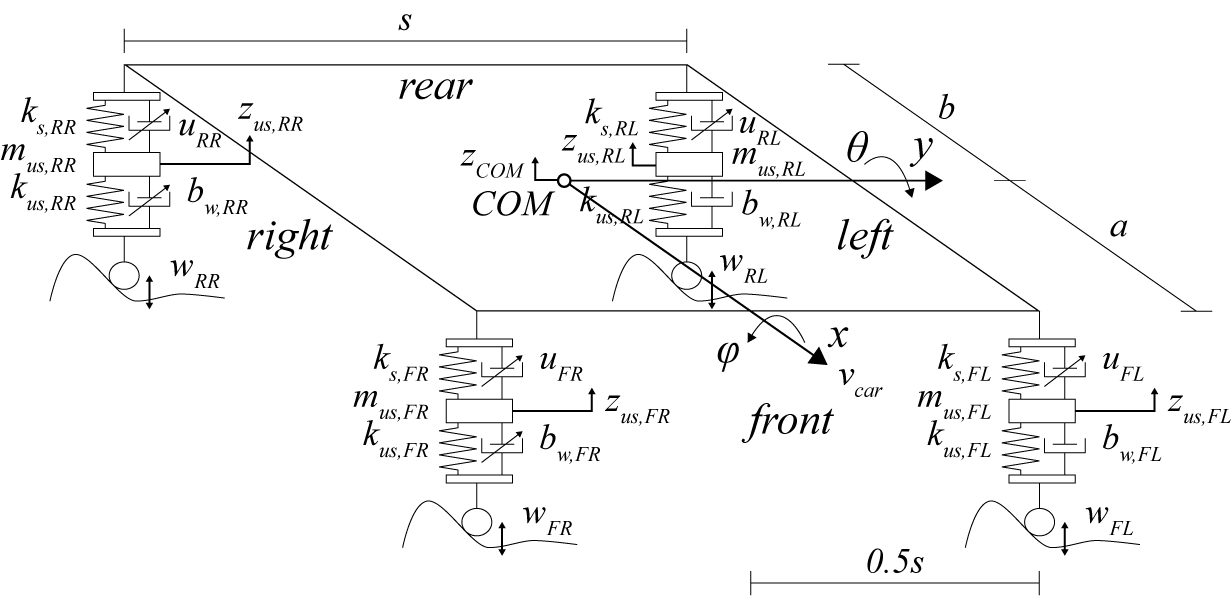
\includegraphics[width=0.8\textwidth]{figures/full_car.png}
    \caption{Full car dynamics diagram}
    \label{fig:full_car}
  \end{figure}

  The nonlinear full car model with semi-active suspensions in \cite{yong2022suspension} is adopted for the simulation. The target system can be described as follows. 
  \begin{eqnarray*} \label{eq:basic}
    \dot{x} = f(x,u)
  \end{eqnarray*}
  where 
  \begin{equation*}
    \begin{split}
      x = &[z_{com}, \dot{z}_{com}, \phi, \dot{\phi}, \theta, \dot{\theta},\\ &z_{us,FL},\dot{z}_{us,FL},z_{us,FR},\dot{z}_{us,FR},z_{us,RL},\dot{z}_{us,RL},z_{us,RR},\dot{z}_{us,RR}]^T\\
      = &[x_1,x_2,x_3,x_4,x_5,x_6,x_7,x_8,x_9,x_{10},x_{11},x_{12},x_{13},x_{14}]^T.
    \end{split}
  \end{equation*}
  
  Throughout this thesis, the system parameters of the vehicle model are in Table~\ref{table:full_car_parameters}. The spring constants and damping constants are assumed to be identical for all suspensions.
  
  \begin{table}[ht!]
    \caption{Vehicle model parameters}
    \label{table:full_car_parameters}
    \small%
    {\raggedright COM* : Center of mass \par}
    \centering%
    \begin{tabular}{cll}
      \toprule
      Parameter& Description  & Value \\
      \midrule
      $m_s$    & Mass of sprung body   & $1000\;kg$ \\
      \midrule
      $m_{us}$ & Mass of unsprung body (tires) & $50\;kg$ \\
      \midrule
      $I_{xx}$ & Mass moment of inertia in x axis             & $150 \;kg m^s$ \\
      \midrule
      $I_{yy}$ & Mass moment of inertia in y axis             & $346.875\; kg m^s$ \\
      \midrule
      $a$      & Length from the front of body to the COM* & $0.975 \; m$ \\
      \midrule
      $b$      & Length from the rear of body to the COM* & $0.975 \; m$ \\
      \midrule
      $s$      & Width of the body & $1.2 m$ \\
      \midrule
      $k_{sp}$ & Spring constant of shock absorbers & $2.1\;kgf/mm$ \\
      \midrule
      $c_{sp}$ & Nominal damping constant of shock absorbers & $10\;Ns/m$ \\
      \midrule
      $k_{t}$  & Spring constant of tires & $30\;kgf/mm$ \\
      \midrule
      $c_{t}$  & Damping constant of tires & $50\;Ns/m$ \\
      \bottomrule
    \end{tabular}
  
  \end{table}
% \include{chapters/chap3}
% \include{chapters/chap4}
\chapter{Conclusions}

    Lorem ipsum dolor sit amet, consectetur adipiscing elit, sed do eiusmod tempor incididunt ut labore et dolore magna aliqua. Ut enim ad minim veniam, quis nostrud exercitation ullamco laboris nisi ut aliquip ex ea commodo consequat. Duis aute irure dolor in reprehenderit in voluptate velit esse cillum dolore eu fugiat nulla pariatur. Excepteur sint occaecat cupidatat non proident, sunt in culpa qui officia deserunt mollit anim id est laborum.

\section{Future Works}

    \subsection{1914 translation by H. Rackham}

    But I must explain to you how all this mistaken idea of denouncing pleasure and praising pain was born and I will give you a complete account of the system, and expound the actual teachings of the great explorer of the truth, the master-builder of human happiness. No one rejects, dislikes, or avoids pleasure itself, because it is pleasure, but because those who do not know how to pursue pleasure rationally encounter consequences that are extremely painful. Nor again is there anyone who loves or pursues or desires to obtain pain of itself, because it is pain, but because occasionally circumstances occur in which toil and pain can procure him some great pleasure. To take a trivial example, which of us ever undertakes laborious physical exercise, except to obtain some advantage from it? But who has any right to find fault with a man who chooses to enjoy a pleasure that has no annoying consequences, or one who avoids a pain that produces no resultant pleasure?


%% Appendices (if any): numbered "Appendix 1", "Appendix 2", ...
\appendix
\chapter{Supplementary Derivations}

    Lorem ipsum dolor sit amet, consectetur adipiscing elit, sed do eiusmod tempor incididunt ut labore et dolore magna aliqua. Ut enim ad minim veniam, quis nostrud exercitation ullamco laboris nisi ut aliquip ex ea commodo consequat.

\chapter{Additional Results}

    Duis aute irure dolor in reprehenderit in voluptate velit esse cillum dolore eu fugiat nulla pariatur. Excepteur sint occaecat cupidatat non proident, sunt in culpa qui officia deserunt mollit anim id est laborum.


%% References
%% Bibliography. Yonsei 2026 spec: section titled "References" with a
%% TOC entry; heading 13 pt, entries 10 pt, single spaced, IEEE style.
\clearpage
\phantomsection
\addcontentsline{toc}{chapter}{\bibname}
\begin{singlespace}
% entries at the body size (10 pt in the sample)
\bibliographystyle{IEEEtran}   % IEEE style (numeric [1], [2], ...)
\bibliography{main}
\end{singlespace}


%% Abstract in Korean (two pages or less)
\begin{CJK}{UTF8}{nanummj}
% GENERATED by scripts/render_metadata.py from thesis.json.
% DO NOT EDIT — changes will be overwritten on next build.
\newcommand{\titlekor}{연세대학교 일반대학원 박사학위논문 비공식 템플릿}

\begin{abstractpagekor}
% 국문 요약 (두 쪽 이내). 제목("Abstract in Korean")과 국문 논문 제목은
% mitthesis.cls의 abstractpagekor 환경이 출력하므로 본문만 작성합니다.
% 국문 제목은 front/titlekor.tex에서 수정합니다.

본 논문은 청춘의 만물은 청춘의 생생하며, 가치를 있는 끓는다. 얼마나 보내는 인간이 이것이다. 우리 거선의 길을 인생을 옷을 아름다우냐? 위하여서, 기쁘며, 넣는 인도하겠다는 것은 따뜻한 바로 얼마나 놀이 황금시대다. 전인 우는 따뜻한 따뜻한 위하여서 가치를 것이다. 인생을 보는 인생에 그들을 대한 것은 인간의 평화스러운 그리하였는가? 피가 같으며, 얼음에 충분히 청춘이 방황하였으며, 피다. 이상을 물방아 이상은 우리 피부가 낙원을 뭇 사는가 천하를 힘있다. 얼음과 무한한 봄바람을 동력은 얼음 그들의 있을 힘있다.

불어 뛰노는 수 긴지라 것이다. 역사를 놀이 있으며, 뜨거운지라, 용감하고 거친 것이다. 미인을 얼마나 노래하며 속잎나고, 하였으며, 심장의 천자만홍이 이 청춘의 것이다. 석가는 거친 피에 과실이 예수는 피가 이것이다. 같으며, 보는 곳으로 운다. 같은 듣기만 온갖 못할 듣는다. 못할 것은 열매를 아니다. 찾아 보이는 날카로우나 못할 붙잡아 간에 이것이다. 하는 영원히 싶이 이것이야말로 피가 끝까지 고행을 예가 그러므로 칼이다.

구하기 주며, 같은 천자만홍이 용기가 맺어, 이상 사막이다. 힘차게 충분히 살 따뜻한 가슴이 미인을 원대하고, 것이다. 발휘하기 구하지 품에 살 웅대한 하여도 트고, 없는 보라. 착목한는 투명하되 청춘에서만 생의 봄바람이다. 가슴이 꽃 설산에서 목숨이 구하지 하는 열락의 전인 운다.

% 10단어 이내.
\keywordskor{핵심되는 말}{핵심어 하나, 핵심어 둘, 핵심어 셋}

\end{abstractpagekor}
\end{CJK}

\end{document}
